\section{Spektraleigenschaften von Graphen}

In diesem Kapitel wollen wir die in Abschnitt \ref{sss:ewgraph} behandelten Themen weiter vertiefen. Insbesondere werden wir einen Zusammenhang zwischen Krauszzerlegungen und den Eigenwerten eines Graphen herstellen. Da spezielle Krauszzerlegungen von Graphen (n"amlich diejenigen mit Minimalgrad mindestens $2$) in Zusammenhang mit Vermutung \ref{con:efl} stehen, werden wir hier eine alternative Herangehensweise an die Erd\H{o}s-Faber-Lov\'asz Vermutung finden.
\subsection{Krauszzerlegungen und Eigenwerte}
\begin{theorem}
  \label{thm:KrauszEigenwerte}
  Seien $G$ ein Graph mit $V(G)=\{v_1,\dots,v_n\}$ und $\mathcal K=\{K^1,\dots,K^p\}$ eine Krauszzerlegung von $G$ mit $\delta(\mathcal K) \geq d \geq 2$. Desweiteren sei $d_i = d_{\mathcal{K}}(v_{i})$ f"ur $1\leq i \leq n$. 
  Dabei w"ahlen wir die Eckennummerierung so, dass $d_1 \geq d_2 \geq \dots \geq d_{n}$ ist.
  Dann gelten folgende Aussagen : 
  \begin{enumerate}[label=\rm{(\alph*)}]
    \item $\lambda_i(G) \geq -d_{n-i+1}$ f"ur $1\leq i \leq n$.
    \item $\lambda_{p+1}(G) \leq -d$ falls $p < n$ ist.
  \end{enumerate}
\end{theorem}

\begin{proof}
  Zun"achst zeigen wir (a). Es sei $A=A(G)$ die Adjazenzmatrix von $G$ und $D = \operatorname{diag}(d_1,\dots,d_n)$. Definiere $B\in\R^{n\times p}$ als die Inzidenzmatrix von $\mathcal K$, d.h. $$B_{ij} = \begin{cases}
    1 & \text{falls } v_i \in K^j \\ 0 & \text{falls }v_i \notin K^j
  \end{cases}$$ 
  Nun betrachten wir $M=BB^{T}$. Die Matrix $M\in \Rnn$ ist symmetrisch und es gilt
  \[
    M_{ij} = \sum\limits_{k=1}^{p}B_{ik}B^{T}_{kj} = \sum\limits_{k=1}^{p}B_{ik}B_{jk}.
  \]
  Seien $1\leq i < j \leq n$. Da $B$ die Inzidenzmatrix von $\mathcal{K}$ ist, gilt  $$ B_{ik} B_{jk} = 1 \Leftrightarrow B_{ik} = 1 \text{ und } B_{jk} = 1 \Leftrightarrow v_i,v_j \in K^{k}.$$ Ist $v_iv_j \in E(G)$, so kommt die Kante $v_iv_j$ in genau einem $K\in \mathcal{K}$ vor, d.h. es gibt genau ein $k\in \left\{ 1,\dots,p \right\}$ f"ur das $B_{ik}$ und $B_{jk}$ gleich $1$ sind. Ist $v_iv_j\notin E(G)$, so kommt die Kante $v_iv_j$ auch nicht in einem der Graphen der Krauszzerlegung vor.
  Also ist f"ur alle $k\in \left\{ 1,\dots, p \right\}$ $B_{ik}B_{jk} = 0$. Folglich ist $M_{ij}=1$ genau dann, wenn $v_iv_j\in E(G)$ gilt. Also ist $M_{ij} = A_{ij}$.
  Sei nun $1\leq i \leq n$. Dann gilt f"ur die Diagonaleintr"age $M_{ii}$ der Matrix $M$:
  \[
    M_{ii} = \sum\limits_{k=1}^{p}B_{ik}B_{ik} = \sum\limits_{k=1}^{p} B_{ik}.
  \]
  Die Gleichung $B_{ik}=1$ gilt genau dann, wenn $v_i \in K^k$ ist. Folglich ist $M_{ii}= d_{\mathcal{K}}(v_i)= d_i$. Damit gilt $M=A+D$. Au{\ss}erdem ist die Matrix $M=BB^{T}$ nach Satz \ref{prop:psdmatrix} positiv semidefinit.
  Folglich ist $A- (-D)$ positiv semidefinit und es folgt mit Lemma \ref{lem:evpsddif}, dass 
  \begin{equation*}
    \lambda_i(G) = \lambda_i(A) \geq \lambda_i(-D) = -d_{n-i+1}
  \end{equation*}
  f"ur alle $1 \leq i \leq n$ gilt. 
  Damit ist (a) gezeigt.

  Nun zeigen wir (b). Sei $p<n$. Da $\operatorname{rang}(M)= \operatorname{rang}(B) \leq p$ ist, gilt dann  $\lambda_{p+1}(M) = 0$. Mit Satz \ref{thm:weylineq} folgt dann, dass
  \begin{align*}
    \lambda_{p+1}(A) + d \leq \lambda_{p+1}(A) + d_{n} = \lambda_{p+1}(A) + \lambda_{n} (D) \leq \lambda_{p+1} (M) = 0
  \end{align*}
  gilt.
  Durch Umstellen erhalten wir die gew"unschte Ungleichung.
\end{proof}

Wir wollen nun eine Folge von Graphenparametern definieren. Seien dazu $d\in\N$ und $G$ ein Graph. Wir bezeichnen mit $\xi_{d}(G)$ die Anzahl aller Eigenwerte von $G$, welche gr"o{\ss}er als $-d$ sind. Damit ist also 
$$\xi_{d}(G) = |\set{i}{\lambda_i(G) > -d}|.$$ 
Dieser ist ein Graphenparamter, da nach Lemma \ref{lem:GraphEigenwerte} isomorphe Graphen dasselbe Spektrum besitzen und somit $\xi_d $ zwei isomorphen Graphen dieselbe nat"urliche Zahl zuordnet. 
Insbesondere gilt (falls $G\neq \varnothing$)
$$\xi_{d}(G) \geq k \Leftrightarrow \lambda_{k}(G) > -d \text{ und } \xi_{d}(G) < k \Leftrightarrow \lambda_{k}(G) \leq -d $$ f"ur alle $1 \leq k \leq n$.

\begin{lemma}
  Seien $G$ ein Graph und $d\in \N$. Dann gelten f"ur den Graphenparameter $\xi_d$ folgende Aussagen:
  \begin{enumerate}[label={\rm(\alph*)}]
    \item Ist $H$ ein induzierter Untergraph von $G$, so gilt $\xi_{d}(H) \leq \xi_{d}(G)$.
    \item Ist $d\geq 2$, so gilt $\omega(G) \leq \xi_{d}(G)$.
    \item $\alpha(G) \leq \xi_{d}(G)$. 
    \item Ist $v\in V(G)$ eine Ecke von $G$, so gilt $\xi_{d}(G) \leq \xi_{d}(G-v) +1$.
    \item Ist $d'\in\N$ mit $d \leq d'$, so gilt $\xi_{d}(G) \leq \xi_{d'}(G)$.
  \end{enumerate}
  \label{lem:xieigenschaften}
\end{lemma}

\begin{proof}
  Wir zeigen zun"achst (a). Sei $\xi_{d}(H) = l$. Folglich ist $\lambda_{l}(H) > -d$ und wir erhalten mit Lemma \ref{lem:InterlacingGraphen}, dass $\lambda_{l}(G) \geq \lambda_{l}(H) > -d$ gilt. Deswegen ist $\xi_{d}(G) \geq l = \xi_{d}(H)$. Also gilt (a).

  Um (b) und (c) zu zeigen, seien $p = \omega(G)$ und $q=\alpha(G)$. Nach Korollar \ref{cor:alphaomegaEigenwerte} ist dann $\lambda_{p}(G) \geq -1$ und $\lambda_q(G) \geq 0$ und deswegen $\xi_{d}(G) \geq p = \omega(G)$ f"ur $d \geq 2$ und $\xi_{d}(G) \geq q = \alpha(G)$ f"ur alle $d \in \N$. 

  F"ur den Beweis von (d) w"ahlen wir eine beliebige Ecke $v$ von $G$. Dann ist $G-v$ ein induzierter Untergraph von $G$ der Ordnung $|G|-1$. Sei $l=\xi_{d}(G-v)$. Ist $l= |G|-1$, so ist nichts zu zeigen, da $\xi_d(G)$ nach oben durch $|G|$ beschr"ankt ist. Andernfalls ist $l< |G| -1$. 
  Dann ist $\lambda_{l}(G-v) > -d$ und $\lambda_{l+1}(G-v) \leq -d$. Nun folgt mit Lemma \ref{lem:InterlacingGraphen} f"ur $k=1$, dass $$\lambda_{l+2}(G) \leq \lambda_{l+1}(G-v) \leq -d$$ ist. Deswegen ist $\xi_{d}(G) \leq l+1 = \xi_{d}(G-v) +1$. Damit ist (d) bewiesen.

  Aussage (e) gilt, da die Eigenwerte eines Graphen fallend geordnet sind.
\end{proof}

Mit Satz \ref{thm:KrauszEigenwerte} erhalten wir einige Aussagen "uber Krauszzerlegungen und den Parameter $\xi_{d}$ von $G$.

\begin{corollary}
  Ist $G$ ein Graph der Ordnung $n$, so gilt $$\xi_{d}(G) \geq | \set{v}{v\in V(G), d_{G}(v) < d}|$$
  f"ur alle $d\in \N$. 
  \label{cor:xiorderschranke}
\end{corollary}
\begin{proof}
  Es sei $\mathcal{K}= \set{G[\{u,v\}]}{uv\in E(G)}$ die Krauszzerlegung von $G$ welche nur aus den Kanten von $G$ besteht und $$l = |\set{v}{v\in V(G), d_{G}(v) < d}|.$$ 
  Desweiteren sei $V(G) = \{ v_1,v_2,\dots , v_n\}$ eine Nummerierung der Kanten, sodass die Gradfolge $d_i = d_{G}(v_i)$, f"ur $1\leq i \leq n$ fallend in $i$ sind. 
  Es gilt $d_{\mathcal{K}}(v) = d_{G}(v)$ f"ur alle Ecken $v$ von $G$ . Dann ist $d_{n-l+1} < d$. Nun folgt aus Satz \ref{thm:KrauszEigenwerte}, dass
  $$\lambda_{l}(G) \geq - d_{n-l+1} > -d$$
  gilt. Also ist $\xi_{d}(G) \geq l$. 
\end{proof}

\begin{corollary}
  \label{cor:Korollar1}
  Seien $G$ ein Graph und $H$ ein induzierter Untergraph von $G$. Dann ist $\kappa_{d}(G) \geq \xi_{d}(H)$.
\end{corollary}

\begin{proof}
  Angenommen, es gilt $p = \kappa_{d}(G) < q=\xi_d(H)$. Dann gibt es  eine Krauszzerlegung $\mathcal{K}$ von $G$ mit $|\mathcal{K}| = p$ und $\delta(\mathcal{K}) \geq d$. 
  Aus Satz \ref{thm:KrauszEigenwerte} folgt, dass $\lambda_{q}(G) \leq \lambda_{p+1}(G) \leq -d $ gilt, da $p+1 \leq q \leq |G|$ ist und die Eigenwerte eines Graphen fallend geordnet sind. 
  Dann ist aber auch $\xi_{d}(G) < q$, im Widerspruch zu $\xi_{d}(G) \geq \xi_{d}(H) \geq  q$ (siehe Lemma \ref{lem:xieigenschaften}). Folglich ist $\kappa_2(G) \geq q$.
\end{proof}

\begin{corollary}
  \label{cor:LineGraphWald}
  Seien $G$ ein Graph und $H$ ein induzierter Untergraph von $G$. Ist $H$ Kantengraph eines Waldes, so gilt 
  $\kappa_{2}(G)\geq \left|H\right|$.
\end{corollary}

\begin{proof}
  Ist $\delta(G) \leq 1$, so ist nichts zu zeigen, da dann mit Lemma \ref{lm:krauszexistenz} folgt, dass $\kappa_2(G) = \infty$ ist.
  Sei sonst $q = |H|$. Da $H$ Kantengraph eines Waldes ist, folgt $\lambda_{q}(H) > -2$ aus Korollar \ref{cor:linegraphwald}. Also ist $\xi_{2}(H) = |H|$.
  Dann ist mit Korollar \ref{cor:Korollar1} $\kappa_{2}\left( G \right) \geq \left| H\right|$.
\end{proof}

\begin{corollary}
  Ist $G$ ein Graph so gilt $\omega\left( G \right)\leq \kappa_{2}\left( G \right)$ und $\alpha\left( G \right)\leq \kappa_{2}\left( G \right)$.
  \label{cor:alphaomegakrausz}
\end{corollary}

\begin{proof}
  Aus Lemma \ref{lem:xieigenschaften} und Lemma \ref{cor:Korollar1} folgt
  \begin{align*}
    \omega(G) &\leq \xi_{2}(G) \leq \kappa_{2}(G) \\
    \alpha(G) &\leq \xi_{2}(G) \leq \kappa_{2}(G) 
  \end{align*}
  und damit die Behauptung.
\end{proof}

Der folgende Korollar wurde bereits von Klotz \cite{Klotz89} gezeigt. Wir erhalten "uber die Krauszzerlegung und Korollar \ref{cor:LineGraphWald} jedoch einen eleganten Beweis.
\begin{corollary}[Klotz]
  Es sei $n \geq 3$. Dann gilt $\kappa_{2}\left( K_n \right) = n$.
\end{corollary}

\begin{proof}
  Um zu sehen, dass $\kappa_{2}(K_n) \leq n$ ist, w"ahlen wir eine Ecke $v$ von $K_n$. 
  Sei $$\mathcal{K} = \{ K_n - v\} \cup \set{K_n[u,v]}{u\in V(K_n), u\neq v}.$$ Dann besteht $\mathcal{K}$ aus einem $K_{n-1}$ und $n-1$ vollst"andigen Graphen der Ordnung $2$. 
  Au{\ss}erdem ist $|\mathcal{K}| = n$ und $\mathcal{K}$ ist eine Krauszzerlegung von $K_n$. Jede Ecke von $K_n$ kommt in mindestens zwei Graphen aus $\mathcal{K}$ vor. Also ist auch $\delta(\mathcal{K}) \geq 2$. 
  Damit ist $\kappa_{2}(K_n) \leq n$. Es bleibt also zu zeigen, dass $\kappa_{2}(K_n) \geq n$ ist. Daf"ur geben wir mehrere Beweise an.
  Mit Hilfe von Korollar \ref{cor:LineGraphWald} folgt die Behauptung, da $K_n$ der Kantengraph von $K_{1,n}$ ist.
  Einen zweiten Beweis erhalten wir mit Korollar \ref{cor:alphaomegakrausz}, da $n = \omega(K_n) \leq \kappa_{2}(K_n)$ ist.
\end{proof}


Um die Erd\H{o}s--Faber--Lov\'asz Vermutung zu beweisen, gen"ugt es zu zeigen, dass jeder Graph $G$ die Ungleichung $$\chi(G) \leq \xi_{2}(G)$$ erf"ullt. Dann gilt mit Korollar \ref{cor:Korollar1} $$\chi(G) \leq \kappa_{2}(G),$$  woraus mit Satz \ref{thm:MainTheorem} dann Vermutung \ref{con:efl} folgt. Wir gelangen also zur folgenden Vermutung.
\begin{conjecture}
  Ist $G$ ein Graph so gilt $\chi(G) \leq \xi_{2}(G)$.
  \label{con:maincon}
\end{conjecture}

Eine M"oglichkeit dies zu zeigen, w"are zu beweisen, dass $\xi_2$ ein Szekeres-Wilf-Paramter ist. Die Eigenschaft (S1) ist nach Lemma \ref{lem:xieigenschaften} erf"ullt. Mit Hilfe von Maple gelang es jedoch einen Graphen $G$ zu finden, f"ur welchen $\xi_{2}(G) < \delta(G) + 1$ ist. 

Es ist jedoch m"oglich, die chromatische Zahl durch eine Funktion von $\xi_2$ nach oben zu beschr"anken, wie der folgende Satz zeigt. Dazu ben"otigen wir einen weiteren Parameter, $\beta$, welcher f"ur einen Graphen $G$ wie folgt definiert ist:
$$\beta(G) = \max\set{|H|}{H\unlhd G, \lambda_{min}(H) > -2}.$$
Eine \DF{dominierende Menge} in $G$ ist eine Menge von Ecken $X$ von $G$ derart, dass jede Ecke in $V(G)\setminus X$ einen Nachbarn in $X$ besitzt. 
Die \DF{Dominierungszahl} $\gamma(G)$ ist die kleinste nat"urliche Zahl $k$, sodass $G$ eine dominierende Menge der M"achtigkeit $k$ besitzt. 
Sei $H$ ein induzierter Untergraph der Ordnung $\beta(G)$ von $G$ dessen Eigenwerte alle gr"o{\ss}er als $-2$ sind. Ist dann $V(H)$ keine dominierende Menge von $G$, so finden wir eine Ecke $v\in V(G) \setminus V(H)$ welche mit keiner Ecke von $H$ benachbart ist.
Dann ist $H'=G[V(H)\cup \{v\}]$ ein induzierter Untergraph von $G$. F"ur diesen gilt $\lambda_{min}(H') = \min\{\lambda_{min}(H), 0\} > -2$ und $|H'| > \beta(G)$ wegen Beispiel \ref{ex:disjointunion}, was unm"oglich ist.
Also ist $V(H)$ eine dominierende Menge und wir finden $\gamma (G) \leq \beta(G)$. 

\begin{theorem}
  Es existiert eine Funktion $f:\N^{2} \to \N$, sodass f"ur alle Graphen $G$ mit $\beta(G)\leq p$ und $\omega(G) \leq q$ gilt $\chi(G) \leq f(p,q) $. 
  \label{lem:funktionxilemma}
\end{theorem}
\begin{proof}
  Es sei $f:\N^{2}\to \N$ die wie folgt rekursiv definierte Funktion:
  $$f(p,q) = \begin{cases}
    1 & \text{ falls } q = 1 \\
    1+p\cdot f(p,q-1) & \text{ falls } q \geq 2.
  \end{cases}$$
  Wir behaupten nun, dass f"ur alle Graphen $G$ mit $\beta(G) \leq p$ und $\omega(G)  \leq q$ gilt $\chi(G) \leq f(p,q)$. 

  Wir beweisen die Aussage durch Induktion nach $q$. F"ur $q=1$ gilt dann $\omega(G) \leq  1$ und deswegen ist $\chi(G) \leq 1 = f(p,1)$. Somit gilt die Aussage f"ur $q=1$. 
  Sei nun $q \geq 2$ und $G$ ein Graph mit $\beta(G) \leq p$ und $\omega(G) \leq q$. Ist $\omega(G) \leq q-1$, so folgt die Behauptung aus der Induktionsvoraussetzung und der Tatsache, dass $f(p,q-1) \leq f(p,q)$ ist. 
  Andernfalls ist $\omega(G) = q$.
  Dann hat $G$ einen induzierten Untergraphen $H$ der Ordnung $l=\beta(G)$ f"ur den $\lambda_{min}(H) > -2$ ist. F"ur $v\in V(H)$ sei $N_v = \set{u\in V(G)}{uv\in E(G)}$, die Menge der Nachbarn von
  $v$ in $G$. Dann ist $\omega(G[N_v]) \leq \omega(G) -1 $, da sonst $G[N_v\cup \{v\}]$ einen vollst"andiger Graphen der Ordnung $q+1$ enth"alt, was nicht m"oglich ist, da $\omega(G) \leq q$ ist. Au{\ss}erdem gilt $\beta(G[N_v]) \leq \beta(G)$, da jeder induzierte Untergraph von $G[N_v]$ wieder ein induzierter Untergraph von $G$ ist. Wegen der Induktionsvorraussetzung folgt dann, dass $\chi(G[N_v]) \leq f(p,q-1)$ ist. 
  Wir setzen $$N = V(G) \setminus \bigcup\limits_{v\in V(H)} N_v$$ 
  und zeigen, dass $G[N]$ kantenlos ist. W"are dem nicht so, so existiert eine Kante $uv\in E(G[N])$. 
  Dann kommen beide Ecken nach Definition von $N$ nicht in $V(H)$ vor. 
  Also gilt $u,v\notin V(H)$ und weder $u$ noch $v$ ist mit einer Ecke aus $H$ benachbart. Wir betrachten den Graphen $$H' = G[V(H) \cup \{u,v\}].$$ Dieser ist ebenfalls ein induzierter Untergraph von $G$ mit $|H'| > |H|$. Da er die disjunkte Vereinigung von $H$ und einem vollst"andigen Graphen der Ordnung $2$ ist, ist das Spektrum von $H'$ die Vereinigung des Spektrums von $H$ und $(1,-1)$ (siehe Beispiel \ref{ex:disjointunion}). Insbesondere ist $$\lambda_{min}(H') = \min \{\lambda_{min}(H),1,-1\} > -2.$$ 
  Dies ist ein Widerspruch zur Wahl von $H$. Also ist $G[N]$ kantenlos und folglich gilt $\chi(G[N]) \leq 1$. 
  Wegen der Subadditivit"at der chromatischen Zahl und $|H| \leq \beta(G) \leq p$ gilt dann $$\chi(G) \leq \chi(G[N]) + \sum\limits_{v\in V(H)}\chi(G[N_v]) \leq 1 + |H|f(p,q-1)  \leq 1+p\cdot f(p,q-1)= f(p,q).$$
\end{proof}

Mit dieser Vorarbeit k"onnen wir nun den folgenden Satz beweisen.
\begin{corollary}
  Es gibt eine Funktion $g:\N \to \N$ welche $$\chi(G) \leq g(\xi_{2}(G))$$ f"ur alle Graphen $G$ erf"ullt. 
  \label{thm:funktionxi}
\end{corollary}

\begin{proof}
  Wir zeigen, dass f"ur alle Graphen $G$ die Ungleichung $\beta(G) \leq \xi_{2}(G) $ erf"ullt ist. Dann folgt die Behauptung, indem wir $g(\xi_2(G))=f(\xi_2(G),\xi_2(G))$ setzen, wobei $f$ die Funktion aus Satz \ref{lem:funktionxilemma} ist. Sei also $\beta(G) = l \in \N$. Dann existiert ein induzierter Untergraph $H$ von $G$ mit $|H| = l$ und $\lambda_{min}(H) = \lambda_{l}(H) > -2$. Folglich ist mit Lemma \ref{lem:InterlacingGraphen} $\lambda_l (G) \geq \lambda_{l}(H) > -2$, was $\xi_2(G) \geq l = \beta(G)$ impliziert.
\end{proof}
Da $\beta(G)$ eine untere Schranke f"ur $\xi_{2}(G)$ ist, folgt aus den Vorbemerkungen dieses Satzes, dass die Dominierungszahl $\gamma(G)$ ebenfalls eine untere Schranke f"ur $\xi_{2}(G)$ ist. 
\begin{theorem}
  \label{thm:MainTheorem}
  F"ur $d\in \N$ gelten folgende Aussagen:
  \begin{enumerate}[label=\rm{(\alph*)}]
    \item Ist $G$ ein Graph mit $\chi(G) \leq \xi_{d}(G)$, so gilt $\chi(G) \leq \kappa_{d}(G)$.
    \item Gilt $\chi(G) \leq \xi_{d}(G) $ f"ur alle Graphen $G$, so ist $\chi'(H) \leq |H|$ f"ur jeden linearen Hypergraphen $H$ mit $|e| \geq d$ f"ur alle $e\in E(H)$. 
  \end{enumerate}
\end{theorem}

\begin{proof}
  Aussage (a) folgt aus Korollar \ref{cor:Korollar1}.  
  Wir zeigen nun (b) durch Widerspruch. Angenommen die Behauptung gilt nicht. Dann gibt es einen linearen Hypergraphen minimaler Ordnung mit $|e| \geq d$ f"ur alle $e\in E(H)$ , f"ur welchen $\chi'(H) > |H|$ ist. 
  Wir machen eine Fallunterscheidung bez"uglich dem kleinsten Kantengrad.

  \ncase{1}{$\delta'(H) < d$} Dann besitzt $H$ eine Kante $e$ vom Grad kleiner als $d$. Da $|e| \geq d$ ist und $H$ ein linearer Hypergraph ist, gibt es eine Ecke $v$ von $H$, welche nur in $e$ vorkommt.
  F"ur $H' = H-v$ gilt dann $V(H') = V(H) \setminus \{v\}$ und $E(H') = E(H) \setminus \{e\}$. Auf Grund der Wahl von $H$ ist $\chi'(H') \leq |H'| = |H|-1$. Also k"onnen die Kanten von $H$ mit $|H|$ Farben gef"arbt werden, indem wir $e$ mit einer neuen Farbe f"arben. 
  Dann ist $\chi'(H') \leq |H|$, ein Widerspruch zur Wahl von $H$. 

  \ncase{2}{$\delta'(H) \geq d$} Sei $G=L(H)$ der Kantengraph von $H$. Dann ist $\delta(G) \geq d$. 
  Sei $K^{v} = G[E_{H}(v)]$ f"ur alle $v\in V(G)$. Sei $\mathcal{K}=\left\{ K^{v} \;|\; v \in V(H) \right\}$. 
  Dann ist $\mathcal{K}$ eine Krauszzerlegung von $G$ mit $\delta_{G}(\mathcal{K}) \geq d$. Damit gilt
  \begin{equation*}
    \chi'(H) = \chi(G) \leq \kappa_{d}(G) \leq |\mathcal{K}| = |H|.
  \end{equation*}
  Wobei die erste Ungleichung wegen der Vorraussetzung von (b) gilt.
\end{proof}

\begin{theorem}
  Sei $G$ ein Graph mit $n$ Ecken und $m$ Kanten. Ist $\xi_{d}(G) \leq k$ mit $k,d\in\N$, so ist
  \begin{align}
    2m \geq \frac{d^{2}n(n-k)}{k}.
    \label{eq:xikantenineq}
  \end{align}
  \label{thm:xikantenschranke}
\end{theorem}

\begin{proof}
  Es bezeichne $\lambda = (\lambda_{1}(G),\lambda_{2}(G), \dots , \lambda_{k}(G))\in \R^{k}$ den Vektor der ersten $k$ Eigenwerte von $G$. Dann ist $\lambda_{i}(G) \leq -d$ f"ur $i \geq k+1$, da $\xi_{d}(G) \leq k$ ist.
  Wegen Lemma \ref{lem:evGraph}(a) gilt dann 
  $$
  \sum\limits_{i=1}^{k} \lambda_{i}(G) = - \sum\limits_{i=k+1}^{n} \lambda_{i}(G) \geq d(n-k).
  $$
  Au{\ss}erdem folgt folgende Ungleichung aus Lemma \ref{lem:evGraph}(b):
  $$ \sum\limits_{i=1}^{k} \lambda_{i}(G)^{2} = 2m - \sum\limits_{i=k+1}^{n} \lambda_{i}(G) ^{2} \leq 2m - (n-k)d^{2}.$$
  Aus einer Absch"atzung der $1$- und $2$-Norm auf $\R^{k}$ folgt au{\ss}erdem 
  $$\| \lambda \|_{2} \geq \frac{1}{\sqrt{k}} \|\lambda\|_{1}.$$
  Damit erhalten wir folgende Ungleichung:
  \begin{align*}
    2m - (n-k)d^{2} &\geq \| \lambda \| _{2}^{2} \\
    & \geq \frac{1}{k} \| \lambda \| _1^{2} \\
    & \geq \frac{1}{k} ( \sum\limits_{i=1}^{k} \lambda_{i}(G))^{2} \\
    & \geq \frac{d^{2}}{k}(n^{2}-2nk+k^{2})
  \end{align*}
  Diese Ungleichung k"onnen wir nach $2m$ umstellen:
  \begin{align*}
    2m \geq d^{2}\frac{n^{2}-2nk + k^{2}+ nk - k^{2} }{k} = d^{2}\frac{n^{2}-nk}{k} = \frac{d^{2}n(n-k)}{k}
  \end{align*}
  Damit ist die Behauptung gezeigt.
\end{proof}
Damit erhalten wir folgende Aussage "uber einen Graphen $G$: Besitzt $G$ nur eine geringe Anzahl von Eigenwerten, die gr"o{\ss}er als $-d$ sind, so muss $G$ viele Kanten besitzen. Besitzt ein Graph $G$ der Ordnung $n$ zum Beispiel nur einen Eigenwert, welcher gr"o{\ss}er als $-1$ ist, so muss $G$ ein vollst"andiger Graph sein. 
Dies erhalten wir, da $\binom{n}{2}$ eine obere Schranke f"ur die Zahl der Kanten $m$ eines Graphen ist. Setzen wir in Gleichung (\ref{eq:xikantenineq}) dann $d=1, k=1$, so erhalten wir 
\begin{equation*}
  n(n-1) \geq 2m \geq n(n-1).
\end{equation*}
Deswegen muss  $G$ alle m"oglichen Kanten enthalten.
\subsection{Schranken f"ur $\kappa_d(G)$}

Wir wollen nun zwei Schranken f"ur $\kappa_{d}(G)$ angeben. Das folgende Lemma folgt sofort aus Lemma \ref{lm:krauszexistenz}. 
\begin{lemma}
  Ist $\delta(G) \geq d$, so ist $\kappa_{d}(G) \leq |E(G)|$. 
\end{lemma}

\begin{theorem}
  Sei $G$ ein Graph der Ordnung $n$ und $d\in \N$. Dann gilt:
  \begin{align*}
    \kappa_{d}(G) &\geq \frac{nd}{\lambda_{1}(G) +d}.
    %\JJambda_n(A) \leq -d 
  \end{align*}
  \label{thm:kappaineq1}
\end{theorem}

\begin{proof}
  Ist $\kappa_{d}(G) = \infty$, so ist nichts zu zeigen. Sei sonst $V(G) = \{v_1,v_2,\dots, v_n\}$ eine Nummerierung der Ecken von $G$.  

  \ncase{1}{$\kappa_{d}(G) \geq n$} Da $\lambda_{1}(G) \geq 0$ erhalten wir $\lambda_{1}(G) + d \geq d$ und somit $1\geq \frac{d}{\lambda_{1}(G) +d}$. Daraus folgt 
  \begin{align*}
    \kappa_{d}(G) \geq n &\geq \frac{nd}{\lambda_{1}(G)+d}.
  \end{align*}

  \ncase{2}{$\kappa_{d}(G) < n$}
  Sei $\mathcal{K}$ eine Krauszzerlegung von $G$ mit $|\mathcal{K}| = \kappa_{d}(G)$ und $\delta_{G}(\mathcal{K}) \geq d$. Seien $d_{i} = d_{\mathcal{K}}(v_i)$. Wir k"onnen annehmen, dass die $d_{i}$ fallend geordnet sind. Sei $B\in \R^{n\times p}$ die Adjanzenzmatrix von $\mathcal{K}$ und $M = BB^{T} = A+D$, wobei $A= A(G)$ und $D = \operatorname{diag}(d_{1},\dots,d_n)$ ist.
  Dann ist $M$ positiv semidefinit und $\operatorname{rang} (M) \leq p = \kappa_{d}(G) < n $. Deswegen ist $\lambda_{p+1}(M) = \dots =\lambda_{n}(M) = 0$. 
  Mit Satz \ref{thm:kyfanineq} und Lemma \ref{lem:evGraph}(a) folgt dann : 
  \begin{align*}
    \sum\limits_{i=1}^{n} \lambda_{i}(D) &=\sum\limits_{i=1}^{n} \lambda_{i}(A) +\sum\limits_{i=1}^{n}  \lambda_{i}(D) \\
    &=\sum\limits_{i=1}^{n} \lambda_{i}(M) =\sum\limits_{i=1}^{p} \lambda_{i}(M) \\
    &\leq \sum\limits_{i=1}^{p} \lambda_{i}(A) +\sum\limits_{i=1}^{p} \lambda_{i}(D).
  \end{align*}
  Daraus folgt 
  $$\sum\limits_{i=p+1}^{n} \lambda_{i}(D) \leq\sum\limits_{i=1}^{p} \lambda_{i}(A)$$ und wir erhalten
  \begin{align*}
    (n-p) d \leq (n-p) \lambda_n(D) \leq \sum\limits_{i=p+1}^{n} \lambda_{i}(D) \leq\sum\limits_{i=1}^{p} \lambda_{i}(A) \leq p\lambda_{1}(A).
  \end{align*}
  Durch Umstellen nach $p$ erhalten wir die gew"unschte Ungleichung.
\end{proof}

\subsection{Chromatische Zahl und Eigenwerte}
Es ist nicht viel "uber den Zusammenhang der chromatischen Zahl eines Graphen und seinen Eigenwerten bekannt. Wir wollen hier auf zwei S"atze verweisen, die Schranken f"ur die chromatische Zahl eines Graphen in Abh"angigkeit des gr"o{\ss}ten bzw. kleinsten Eigenwerts angeben. Die folgende Absch"atzung der chromatischen Zahl nach oben durch den maximalen Eigenwert plus $1$ stammt von Wilf \cite{Wilf67}.

\begin{theorem}[Wilf]
  Ist $G$ ein zusammenh"angender Graph, so gilt: 
  $$\chi(G) \leq \lambda_{1}(G) +1.$$
  Gleichheit tritt nur auf, falls $G$ ein vollst"andiger Graph oder ein ungerader Kreis ist.
  \label{thm:wilfev}
\end{theorem}

\begin{proof}
  Wir zeigen, dass $\lambda_{1}+1$ ein Szekeres-Wilf Parameter ist. Dann folgt die Behauptung wegen Satz \ref{thm:szekereswilf}. Sei dazu $|G| = n \in \N$ und $V(G)= \{v_1,v_2, \dots , v_n \}$ eine Nummerierung der Ecken. 
  Wir beweisen zun"achst (S1). Sei $H$ ein induzierter Untergraph von $G$. Dann ist wegen Lemma \ref{lem:InterlacingGraphen} $\lambda_{1}(H) \leq \lambda_{1}(G)$ und folglich auch $\lambda_{1}(H) +1 \leq \lambda_{1}(G) +1$.
  Wir zeigen nun (S2). F"ur den Rayleigh-Quotienten des Vektors $x\in \R^{n}$, dessen Komponenten alle gleich $1$ sind, gilt dann:
  $$R_{A(G)}(x) = \frac{x^{T}A(G)x}{x^{T}x} = \frac{x^{T}(d_G(v_1),d_G(v_2),\dots, d_G(v_n))^{T}}{n} = \frac{1}{n} \sum\limits_{i=1}^{n} d_G(v_i).$$ 
  Also ist dieser gleich dem durchschnittlichen Eckengrad. Folglich gilt $R_{A(G)}(x) \geq \delta(G)$. Au{\ss}erdem folgt aus Satz \ref{thm:CourantFischer}, dass $\lambda_{1}(G) = \lambda_{1}(A(G)) \geq R_{A(G)}(x)$ ist. Somit ist
  $\lambda_{1}(G) +1 \geq \delta(G) +1$. Damit haben wir (S2) gezeigt. 
  Also ist $\lambda_{1}+1$ ein Szekeres-Wilf Parameter und wegen Satz \ref{thm:szekereswilf} gilt $\chi(G) \leq \lambda_{1}(G) +1 $. 
  Sei nun $G$ ein Graph mit $\chi(G) = \lambda_{1}(G) +1$. Wir m"ussen zeigen, dass $G$ ein ungerader Kreis oder ein vollst"andiger Graph ist.
  Wegen Satz \ref{thm:forbiddencritgraph} gibt es dann einen $k$-kritischen induziereten Untergraphen $H$ von $G$. Wegen Lemma \ref{lem:kritgraph} ist dann $\delta(H) \geq k-1$. Somit gilt 
  $$k-1 = \lambda_{1}(G)  \geq \lambda_{1}(H) \geq \delta(H) \geq k-1$$
  also
  $$\lambda_{1}(G) = \lambda_{1}(H) = \delta(H).$$
  Da $G$ zusammenh"angend ist, kann man mit Satz \ref{thm:zusammenhgraph} zeigen, dass gilt: $G= H$ und $G$ ist regul"ar. Also gilt $\chi(G) = \Delta(G) +1 $. Dann folgt aus dem Satz von Brooks \ref{thm:brooks}, dass $G$ ein vollst"andiger Graph oder ein ungerader Kreis ist. 
\end{proof}

Eine untere Schranke f"ur die chromatische Zahl geht auf Hoffman \cite{Hoffman70} zur"uck (man beachte hierbei, dass $\lambda_{min}(G)$ negativ ist):
\begin{theorem}
  Ist $G$ ein Graph, so gilt:
  $$\chi(G) \geq 1 - \frac{\lambda_{max}(G)}{\lambda_{min}(G)}.$$
  \label{thm:Hoffmanev}
\end{theorem}

\subsection{Graphen mit $\chi \leq \xi_{2}$}

Wir haben bereits gesehen, dass Vermutung \ref{con:maincon} die Erd\H{o}s--Faber--Lov\'asz Vermutung impliziert. Im folgenden Abschnitt wollen wir deswegen Graphen untersuchen, deren chromatische Zahl durch die Anzahl der Eigenwerte, die gr"o{\ss}er als $-2$ sind, beschr"ankt ist.
\begin{remark}
  Es gen"ugt Vermutung \ref{con:maincon} f"ur $k$-kritische Graphen zu zeigen. 
\end{remark}

\begin{proof}
  Gelte Vermutung \ref{con:maincon} f"ur kritische Graphen.
  Sei $G$ ein Graph mit $\chi(G) = k$. Dann enth"alt $G$ nach Satz \ref{thm:forbiddencritgraph} einen $k$-kritischen Untergraphen $H$. F"ur diesen gilt nach Vorraussetzung $$k= \chi(H) \leq \xi_{2}(H).$$ Dann ist aber auch $$ \chi(G) = k \leq \xi_{2}(H) \leq \xi_{2}(G) ,$$ da $H$ ein induzierter Untergraph von $G$ ist (siehe Lemma \ref{lem:xieigenschaften}).  Damit gilt Vermutung \ref{con:maincon} auch f"ur $G$.
\end{proof}

Wir haben bereits in Satz \ref{cor:linegraphwald} gesehen, dass alle Eigenwerte eines Kantengraphen durch $-2$ nach unten beschr"ankt sind. Au{\ss}erdem haben wir in Satz \ref{thm:sachszshgrapheigenwert} die Vielfachheit des Eigenwerts $-2$ eines Kantengraphs bestimmt. Damit l"asst sich nun leicht beweisen, dass Kantengraphen Vermutung \ref{con:maincon} erf"ullen. 
\begin{theorem}
  Sei $G=L(H)$ der Kantengraph eines Graphen $H$ mit $E(H)\neq \varnothing$. Dann gilt $$\chi(G) \leq \xi_2(G).$$
  \label{thm:linegraphconjecture}
\end{theorem}

\begin{proof}
  Wir k"onnen annehmen, dass $H$ zusammenh"angend ist. Sonst betrachten wir die Komponenten $H_1,H_2,\dots,H_\ell$ von $H$ (welche wenigstens eine Kante enthalten). Dann sind $G_i= L(H_i)$ ($1\leq i \leq \ell$) die Komponenten von $G$. Und es gilt $\chi(G) = \max\limits_{1 \leq i \leq \ell} \chi(G_i)$ sowie $\xi_{2}(G) = \xi_{2}(G_1) + \xi_{2}(G_2) + \dots + \xi_{2}(G_\ell)$ (siehe Beispiel \ref{ex:disjointunion}). 

Sei also $H$ ein zusammenh"angender Graph mit $n$ Ecken, $m$ Kanten und $G = L(H)$. Da $E(H) \neq \varnothing$ ist, gilt $n \geq 2$ und wegen Satz \ref{cor:linegraphwald} ist dann $\xi_{2}(G) = |G| - m_G(-2) = m - m_G(-2)$. Ist $H$ bipartit, so folgt aus Satz \ref{thm:konigbip}, dass $\chi(G) = \Delta(H)$ ist.  
  Desweiteren ist dann $m_G(-2) = m-n+1$ (siehe Satz \ref{thm:sachszshgrapheigenwert}). Deswegen ist $\xi_{2}(G) = m - (m-n+1) = n-1$ und es gilt
  $$\chi(G) = \Delta(H) \leq n-1  = \xi_{2}(G).$$
  Ist $G$ nicht bipartit, so ist nach dem Satz von Vizing \ref{thm:Vizing} $\chi(G) \leq \Delta(H) +1$. Aus Satz \ref{thm:sachszshgrapheigenwert} folgt dann $m_G(-2) = m-n$. Folglich ist $\xi_{2}(G) = m - (m-n) = n$. Damit gilt
  $$\chi(G) \leq \Delta(H) +1 \leq n = \xi_{2}(G).$$
  Was zu zeigen war.
\end{proof}
\begin{theorem}
  Sei $G$ ein Graph. Ist $\chi(G) \leq 3$, so gilt $\chi(G) \leq \xi_{2}(G)$.
  \label{thm:chiklein}
\end{theorem}

\begin{proof}
  Sei $n=|G|$. Wir machen eine Fallunterscheidung bez"uglich $k=\chi(G)$.

  \ncase{1}{$k=0$} Dann ist $G=\varnothing$, der leere Graph. Also ist $\chi(G) = 0 = \xi_{2}(G)$. 

  \ncase{2}{$k=1$} Dann ist $n\geq 1$ und $G$ enth"alt keine Kanten. Also ist $G$ ein kantenloser Graph der Ordnung $n$ und mit Lemma \ref{lem:xieigenschaften} folgt
  $$\chi(G) = 1 \leq n = \alpha(G) = \xi_{2}(G).$$

  \ncase{3}{$k=2$} Dann ist $G$ bipartit und $G$ besitzt mindestens eine Kante. Also ist $\omega(G) = 2$ und es folgt aus Lemma \ref{lem:xieigenschaften} dass
  $$\chi(G) = 2 = \omega(G) \leq \xi_{2}(G)$$
  gilt.

  \ncase{4}{$k=3$} Dann ist $G$ nicht bipartit. Deswegen besitzt $G$ nach dem Satz von K"onig einen ungeraden Kreis als Untergraphen. Es sei $C$ ein ungerader Kreis von $G$ minimaler Ordnung. Dann ist $|C| = p \geq 3$. 
  Wir zeigen, dass $C$ ein induzierter Untergraph von $G$ ist. Angenommen, das ist nicht der Fall. Dann exisiteren zwei Ecken $u,v\in V(C)$ mit $uv\in E(G) \setminus E(C)$. Dann besteht $C+uv$ aus zwei Kreisen $C_1$ und $C_2$ welche nur die Kante $uv$ gemeinsam haben. Au{\ss}erdem ist die Ordnung dieser Kreise kleiner als die Ordnung von $C$.
  Ist sowohl $C_1$, als auch $C_2$ von gerader Ordnung, so muss auch $C$ von gerader Ordnung sein, da $|C| = |C_1| + |C_2| -2$ gilt (die einzigen Ecken die $C_1$ und $C_2$ gemeinsam haben sind $u$ und $v$). Also ist einer der beiden Kreise ein ungerader Kreis kleinerer Ordnung als $C$. Das steht aber im Widerspruch zur Wahl von $C$. 
  Also ist $C$ ein induzierter Untergraph von $G$. Au{\ss}erdem ist $C=L(C)$ und $\chi(C) = 3$. Dann folgt aus Lemma \ref{thm:linegraphconjecture} und Lemma \ref{lem:xieigenschaften}, dass 
  $$\chi(G) = 3 = \chi(C) \leq \xi_{2}(C) \leq \xi_{2}(G)$$
  ist.
\end{proof}


Seien $p,r$ zwei nat"urliche Zahlen mit $p\geq 2r-1$. Der \DF{Kneser Graph} $K_{p:r}$ geht auf Kneser \cite{Kneser55} zur"uck und ist der Graph mit Eckenmenge $$V(K_{p:r}) = [\{1,2,\dots,p\}]^{r}$$ und Kantenmenge 
$$E(K_{p:r}) = \left\{ XY\;|\; X,Y \in V(K_{p:r}), X \cap Y = \varnothing \right\}.$$ 
$K_{p:1}$ ist ein vollst"andiger Graph der Ordnung $p$ und $K_{2r-1:r}$ ist ein kantenloser Graph der Ordnung $\binom{2r-1}{r}$.
Der Graph $K_{5:2}$ ist auch als der Petersen Graph bekannt (siehe Abbildung \ref{fig:petersen}).

\begin{figure}[h]
  \centering
  \includegraphics{images/petersen}
  \caption{Der Petersen Graph $K_{5:2}$}
  \label{fig:petersen}
\end{figure}
Kneser gibt in \cite{Kneser55} eine obere Schranke f"ur die chromatische Zahl der Kneser Graphen an. Sp"ater zeigte Lov\'asz \cite{Lovasz78} dass diese Schranke immer angenommen wird.
\begin{theorem}[Lov\'asz]
  Ist $p\geq 2r-1$, so gilt
  $\chi(K_{p:r}) = p-2r+2$. \label{thm:kneserfarbung}
\end{theorem}

Der folgende Satz ist als Satz von Erd\H{o}s-Ko-Rado \cite{ErdosKoRado61} bekannt und gibt die Unabh"angigkeitszahl eines Kneser Graphen an.
\begin{theorem}[Erd\H{o}s-Ko-Rado]
  Ist $p\geq 2r$ und $r \geq 2$, so gilt: 
  $\alpha(K_{p:r})= \binom{p-1}{r-1}$.
  \label{thm:ErdosKoRado}
\end{theorem}

Mit den beiden vorangegangenen S"atzen k"onnen wir nun beweisen, dass Kneser Graphen die Vermutung \ref{con:maincon} erf"ullen.
\begin{proposition}
  Es sei $G=K_{p:r}$ ein Kneser Graph mit $p\geq 2r-1$ und $r \geq 1$. Dann ist $\chi(G) \leq \xi_{2}(G)$. 
\end{proposition}
\begin{proof}
  Sei $\chi(G) = k$. Wir machen eine Fallunterscheidung bez"uglich $r$.

  \ncase{1} {$r=1$} Dann ist $G=K_{p:1}$ ein vollst"andiger Graph der Ordnung $p$. Die Eigenwerte des $K_p$ sind nach Beispiel \ref{ex:vollstgraph} alle gr"o{\ss}er als $-2$. Folglich ist $\chi(G) \leq \xi_{2}(G)$. 

  \ncase{2} {$p > 2r \geq 4 $} Sei $q = \alpha(G)$.  Dann ist nach Satz \ref{thm:ErdosKoRado} $ q = \binom{p-1}{r-1}$ und folglich $ q \geq p-1$. Nach Satz \ref{thm:kneserfarbung} ist $\chi(G) = p-2r+2 < p-2$. Folglich ist $q > \chi(G)$. 
  Dann gilt $$\chi(G) < q = \alpha(G) \leq \xi_{2}(G) $$ wegen Lemma \ref{lem:xieigenschaften}.

  \ncase{3} {$ p = 2r $} Die Ecken von $G$ sind alle $r$-elementigen Teilmengen von $\left\{ 1,\dots,p \right\}$. Da $p=2r$ ist f"ur ein $w\in V(G)$ die einzige benachbarte Ecke ihr Komplement in $\left\{ 1,\dots,p \right\}$. 
  Also hat jede Ecke von $G$ den Grad $1$ und jede Komponente von $G$ ist ein vollst"andiger Graph der Ordnung $2$.
  Nach Beispiel \ref{ex:vollstgraph} und Beispiel \ref{ex:disjointunion} ist dann 
  $$\operatorname{sp} (G) = (\underbrace{1,1,\dots,1}_{\frac{|G|}{2} \text{ mal}} , \underbrace{-1,-1,\dots,-1}_{\frac{|G|}{2} \text{ mal}}). $$
  Daraus folgt dann $\chi(G) \leq |G| = \xi_{2}(G)$.

  \ncase{4}{$p=2r+1$} Dann ist $G$ ein kantenloser Graph. Deswegen ist $\chi(G) = 1$ und $\chi(G) = 1 \leq |G| = \alpha(G) = \xi_{2}(G)$ (siehe Lemma \ref{lem:xieigenschaften}).
\end{proof}
Eine weitere Klasse die Vermutung \ref{con:maincon} erf"ullt, ist die Klasse der perfekten Graphen.

\begin{proposition}
  Sei $G$ ein perfekter Graph. Dann gilt 
  $\chi(G) \leq \xi_{2}(G)$.
\end{proposition}

\begin{proof}
  Da $G$ ein perfekter Graph ist, gilt $\chi(G) = \omega(G)$. 
  Mit Lemma \ref{lem:xieigenschaften} folgt dann $\xi_2(G) \geq \omega(G) = \chi(G)$.
\end{proof}

Planare Graphen sind nach dem Vierfarbensatz \cite{AppelHaken76} mit $4$ Farben f"arbbar. Der nachfolgende Satz garantiert, dass alle planaren Graphen der Ordnung mindestens $7$ mindestens $4$ Eigenwerte besitzen, die gr"o{\ss}er als $-2$ sind.
\begin{proposition}
  Sei $G$ ein planarer Graph mit $|G| \geq 7$. Dann gilt $\xi_{2}(G) \geq 4$.
  \label{prop:planaregraphen}
\end{proposition}

\begin{proof}
  Den Beweis f"uhren wir indirekt. Angenommen, es gibt einen planaren Graphen $G$ mit $|G| \geq 7$ und $\xi_{2}(G) \leq 3$. Sei $n$ die Ordnung von $G$. 
  Aus Satz \ref{thm:xikantenschranke} (f"ur $d=2, k=3$) folgt, dass f"ur die Zahl $m$ der Kanten von $G$ gilt:
  $$2m \geq \frac{4n(n-3)}{3}.$$
  Da $G$ ein planarer Graph ist, gilt zus"atzlich $$ m \leq 3n-6.$$
  Wir erhalten nun durch Umstellen die quadratische Ungleichung $$-2n^{2} +15n -18 \geq 0.$$
  L"osen dieser Ungleichung ergibt $ \frac{3}{2} \leq n \leq 6$, ein Widerspruch zur Vorrausetzung $n\geq 7$.
\end{proof} 
Aus dem vorhergehenden Satz erhalten wir sofort, dass jeder planare Graph die Vermutung \ref{con:maincon} erf"ullt.
\begin{corollary}
  Sei $G$ ein planarer Graph. Dann gilt $\chi(G) \leq \xi_{2}(G) $. 
\end{corollary}
\begin{proof}
  Wir machen eine Fallunterscheidung bez"uglich der chromatischen Zahl $\chi(G)=k$. Auf Grund des $4$-Farbensatzes reicht es dann die F"alle $k\leq 4$ zu betrachten.

  \ncase{1}{$k\leq 3$} Dann folgt $\chi(G) \leq \xi_{2}(G)$ aus Satz \ref{thm:chiklein}.

  \ncase{2}{$k = 4$} $G$ enth"alt nach Satz \ref{thm:forbiddencritgraph} einen $4$-kritischen Untergraphen $G'$. Ist $|G'| \geq 7$, so ist wegen Satz \ref{prop:planaregraphen} $\xi_{2}(G') \geq 4$. Mit Lemma \ref{lem:xieigenschaften} folgt dann $\xi_{2}(G) \geq \xi_{2}(G') \geq 4 = \chi(G)$.
  Ist $|G'| \leq 6$, so folgt aus einem Resultat von Gallai \cite{Gallai63}, dass $G' = K_4$ ist oder $G'$ den Kreis $C_5$ als induzierten Untergraphen enth"alt. Nun folgt aus Lemma \ref{lem:xieigenschaften}, Beispiel \ref{ex:vollstgraph} und Beispiel \ref{ex:kreiseeigenwerte}: $$\xi_{2}(G) \geq \xi_{2}(G') \geq 4 = \chi(G).$$ 
  Was zu zeigen war.
\end{proof}

Nordhaus und Gaddum \cite{NordhausG56} zeigten, dass ein Graph $G$ der Ordnung $n$ und sein Komplement $\overline{G}$ stets die Ungleichung $\chi(G) + \chi(\overline{G}) \leq n+1$ erf"ullen. Au{\ss}erdem bewies Finck \cite{Finck66}, dass Gleichheit in dieser Ungleichung genau dann gilt, wenn $G$ von einem der beiden Graphentypen $F_1$ oder $F_2$ ist. 
Diese sind wie folgt definiert:
Seien $n,p$ zwei nat"urliche Zahlen. 

Ein Graph $G$ geh"ort zum Typ $F_1 (n,p)$, falls $G$ aus einer unabh"angigen Menge $O$ der Ordnung $p$ und einem vollst"andigen Graphen $K$ der Ordnung $n-p+1$ besteht und es genau eine Ecke gibt, welche sowohl in $O$ als auch in $K$ vorkommt. Zwischen $O$ und $K$ d"urfen Kanten verlaufen. 

Ein Graph $G$ geh"ort zum Typ $F_2(n,p)$, falls $G$ aus einem Kreis $C=C_5$, einem vollst"andigen Graphen $K=K_{n-p-5}$ und einer unabh"angigen Menge $O=O_{p}$ besteht. 
Seien $v\in V(C), w\in V(K), u\in V(O)$ beliebig. Dann ist $vw\in E(G), vu\notin E(G) $ und $uw$ kann, muss aber nicht zu $E(G)$ geh"oren.

\begin{theorem}
  Sei $G$ ein Graph der Ordnung $n$. Dann gilt 
  $\xi_{2}(G) + \xi_{2}(\overline{G}) \geq n.$ 
  \label{thm:xikomplement}
\end{theorem}
\begin{proof}
  Seien $\xi_{2}(G) = l$, $A= A(G)$ die Adjazenzmatrix von $G$ und $\overline A = A(\overline{G}) = J-I-A $ die Adjazenzmatrix von $\overline{G}$. 
  Ist $l = n$, so ist nichts zu zeigen. Wir betrachten also den Fall $l< n$. Dann ist $\lambda_{l+1}(A) \leq -2$. Zeigen wir $\xi_{2}(\overline{G}) \geq n-l$, so ist die Behauptung bewiesen. 
  Nach Satz \ref{thm:CourantFischer} ist 
  $$\lambda_{n-l}(\overline{A}) = \max\set{\min\limits_{x\in V , x \neq 0} R_{\overline{A}}(x)}{ V\subseteq \R^n \text{ linearer Unterraum,} \operatorname{dim}(V) =  n-l}.$$
  Ist also $V$ ein linearer Unterraum des $\R^{n}$ der Dimension $n-l$, so gilt $$\lambda_{n-l} (\overline{A}) \geq \min\limits_{x\in V, x\neq 0} R_{\overline{A}(x)}.$$
  Au{\ss}erdem folgt aus Satz \ref{thm:CourantFischer}, dass es einen linearen Unterraum $V$ des $\R^{n}$ der Dimension $n-l$ gibt mit $ \max \limits_{x\in V}R_{A}(x) =\lambda_{l+1} (A)  \leq -2$.
  Insbesondere ist also $R_{A}(x) \leq -2$ f"ur alle $x\in V$.
  Wir betrachten den Rayleigh Quotienten von $\overline{A}$ auf diesem Unterraum. Da $J$ positiv semidefinit ist, gilt f"ur alle $x\in V$ mit $x\neq 0$
  $$R_{\overline{A}}(x) = R_{J}(x) - R_I(x) - R_A(x) \geq  R_J(x) - 1 + 2 = R_J(x) +1  \geq 1.$$
  Dann ist $\lambda_{n-l}(\overline{A}) \geq \min\limits_{x\in V} R_{\overline{A}}(x) \geq 1$. 
  Also ist $\xi_{2}(\overline{G}) \geq n-l$. 
\end{proof}



\begin{theorem}
  Sei $G$ ein Graph. Dann gilt $\chi(G) + \chi(\overline{G}) \leq \xi_{2}(G) +  \xi_{2}(\overline{G})$.
  \label{thm:xichromatisch}
\end{theorem}
\begin{proof}
  Gilt $\chi(G) + \chi(\overline{G}) \leq n$, so ist nach Satz \ref{thm:xikomplement} nichts mehr zu zeigen. Andernfalls ist $G$ entweder vom Typ $F_1$ oder $F_2$. 

  \ncase{1}{$G$ ist vom Typ $F_1(n,p)$} Dann ist $\omega(G) = n-p+1$ und $\omega (\overline{G})=p$. Dann folgt mit Lemma \ref{lem:xieigenschaften}, dass gilt
  $$\xi_{2}(G) + \xi_{2}(\overline{G}) \geq \omega(G) + \omega(\overline{G}) = n+ 1 = \chi(G) + \chi(\overline{G}).$$

  \ncase{2}{$G$ ist vom Typ $F_2(n,p)$} Es sei $C$ der Kreis der Ordnung $5$ in $G$, $K$ der vollst"andige Graph der Ordnung $n-p-5$ in $G$ und $O$ der kantelose Graph der Ordnung $p$ in $G$. Wir betrachten den induzierten Untergraphen $H=G[V(C) \cup V(O)]$. Dann ist $H$ die disjunkte Vereinigung eines kantenlosen Graphen und eines $C_5$. Es gilt $|H| = p+5$ und aus Beispiel \ref{ex:kreiseeigenwerte}, Beispiel \ref{ex:kantenlosergraph} sowie Beispiel \ref{ex:disjointunion} folgt, dass $\xi_{2}(H) = |H|$ ist. 
  F"ur $\tilde{H} = \overline{G} [V(C) \cup V(K)]$ gilt dann nach dem selben Argument $$\xi_{2}(\tilde{H}) = |\tilde{H}| = |V(C)| + |V(K)| = n-p .$$ Dann gilt 
  $$\xi_{2}(G) + \xi_{2}(\overline{G}) \geq \xi_{2}(H) + \xi_{2}(\overline{H}) = p+5 + n -p = n+ 5 > n+ 1 = \chi(G) + \chi(\overline{G}).$$
  Damit ist alles gezeigt.
\end{proof}

\begin{corollary}
  F"ur jeden Graphen $G$ gilt $\chi(G) \leq \xi_{2}(G)$ oder $\chi(\overline G) \leq \xi_{2}(\overline{G})$.
\end{corollary}

\subsection{Haj\'os und Ore Summe}
Haj\'os \cite{Hajos61} bewies 1971, dass jeder Graph mit chromatischer Zahl wenigstens $k$ einen Untergraphen enth"alt, welcher aus vollst"andigen Graphen $K_k$ durch wiederholte Anwendung zweier einfacher Konstruktionen gebildet werden kann. 
Ore \cite{Ore67} bewies ein "ahnliches Resultat, wobei er die beiden Konstruktionen zu einer Konstruktion zusammenfasste. Uruquaht \cite{Urquhart97} zeigte 1997, dass durch beide Methoden diesselbe Graphenklasse erzeugt wird. 

Sei $G$ ein Graph, und seien $u,v$ zwei verschiedene unabh"angige Ecken von $G$. Wir erhalten dann einen neuen Graphen $G'$ indem wir zu $G-u-v$ eine neue Ecke $w$ hinzuf"ugen und diese mit allen Nachbarn von $u$ und $v$ in $G$ durch eine Kante verbinden.
Man sagt dann, dass $G'$ aus $G$ durch \DF{Identifizierung} der unabh"angigen Ecken $u,v$ entsteht (siehe Abbildung \ref{fig:identifizierung}).
\begin{figure}[h]
  \centering
  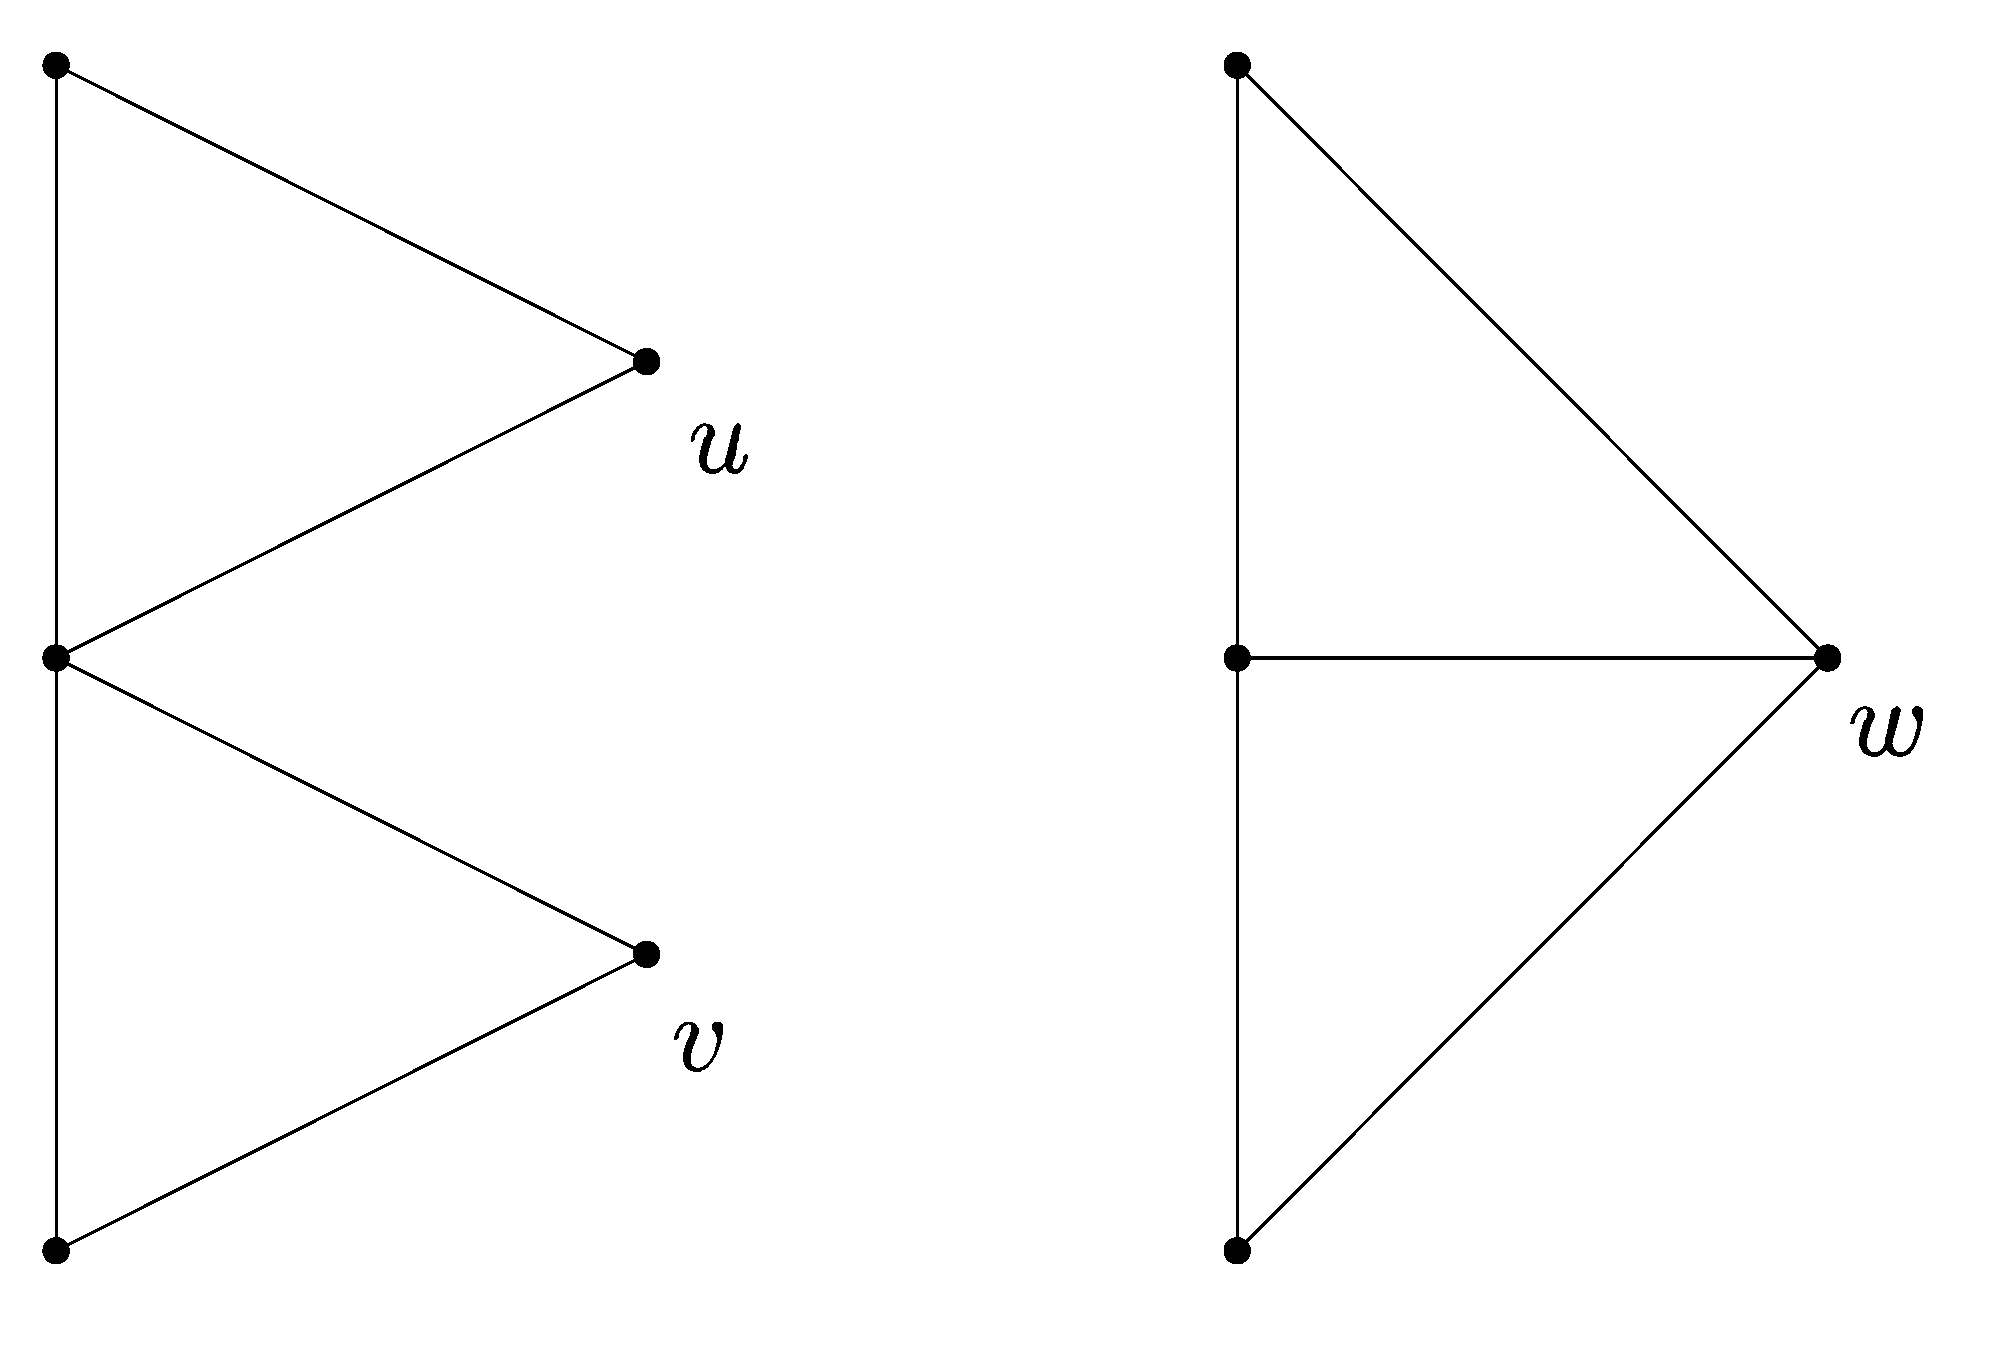
\includegraphics[width=0.5\textwidth]{images/Identifizierung}
  \caption{Identifizierung von $u$ und $v$.}
  \label{fig:identifizierung}
\end{figure}

Seien $G_1, G_2$ zwei nichtleere disjunkte Graphen und $x_1y_1\in E(G_1)$ sowie $x_2y_2 \in E(G_2)$ zwei beliebige Kanten. Die \DF{Haj\'os Summe} von $G_1$ und $G_2$ (bez"uglich $x_1y_1$ und $x_2y_2$) ist derjenige Graph, der entsteht wenn wir $G_1$ und $G_2$ vereinigen, die Kanten $x_1y_1$ und $x_2y_2$ entfernen, die Kante $y_1y_2$ hinzuf"ugen und  die Ecken $x_1$ und $x_2$ identifizieren. 
In Abbildung \ref{fig:HajosSumme} sehen wir die Haj\'os Summe zweier Dreiecke.

\begin{figure}[h]
  \centering
  \includegraphics[width=0.8\textwidth]{images/HajosSumme}
  \caption{Haj\'os Summe von $G_1$ und $G_2$}
  \label{fig:HajosSumme}
\end{figure}
Wir betrachten nun im folgenden f"ur $k\in \N$ die Graphenklasse $\mathcal{H}_k$ der \DF{$k$-Haj\'os konstruierbaren Graphen}. Diese ist die kleinste Klasse von Graphen, welche $K_k$ enth"alt und abgeschlossen ist bez"uglich der Isomorphie von Graphen, der Ha\'os Summe von Graphen und der Identifikation zweier unabh"angiger Ecken. Somit geh"ort $K_k$ zu $\mathcal{H}_k$. Weiterhin geh"ort mit jedem Graphen aus $\mathcal{H}_k$ auch jeder dazu isomorphe Graph zu $\mathcal{H}_k$,
mit je zwei disjunkten Graphen aus $\mathcal{H}_k$ geh"ort auch ihre Haj\'os Summe zu $\mathcal{H}_k$, und mit jedem Graphen aus $\mathcal{H}_k$ geh"ort auch jeder Graph zu $\mathcal{H}_k$, welcher aus $G$ durch die Identifizierung zweier unabh"angiger Ecken gebildet werden kann. 

Eine weitere, der H\'ajos Summe "ahnliche Konstruktion ist die \DF{Ore Summe}. Seien $G_1$ und $G_2$ zwei disjunkte Graphen, $x_1y_1$ eine Kante von $G_1$ und $x_2y_2$ eine Kante von $G_2$. Desweiteren seien $v_1,v_2,\dots,v_r$ unterschiedliche Ecken von $G_1- x_1$ und $u_1,u_2,\dots,u_r$ unterschiedliche Ecken von $G_2- x_2$. 
Wir konstruieren nun die Ore Summe von $G_1$ und $G_2$ aus der H\'ajos Summe von $G_1$ und $G_2$, indem wir zus"atzlich die Ecken $v_i$ mit $u_i$ identifizieren (f"ur $1\leq i \leq r$). Der so entstandene Graph ist dann die Ore Summe von $G_1$ und $G_2$. 

F"ur $k\in \N$ sei $\mathcal{O}_k$ die Klasse der \DF{Ore $k$-konstruierbaren Graphen}. Dies ist die kleinste Klasse von Graphen, welche $K_k$ enth"alt und abgeschlossen ist bez"uglich der Isomorphie von Graphen und der Ore Summe von Graphen.
Der folgende Satz wurde 1997 von Uruquhart  \cite{Urquhart97} bewiesen. Dieser Satz versch"arft fr"uhere Resultate von Haj\'os \cite{Hajos61} und Ore \cite{Ore67}. 
\begin{theorem}[Uruquhart]
  Sei $k\in \N$ und $k \geq 3$. Dann sind die Klassen $\mathcal{H}_k$ und $\mathcal{O}_k$ identisch und ein Graph $G$ geh"ort genau dann zu dieser Klasse, wenn $\chi(G) \geq k$ ist.
  \label{thm:uruquhart}
\end{theorem}

Eine Folgerung aus diesem Satz ist, dass Vermutung \ref{con:maincon} zur folgenden Vermutung "aquivalent ist.
\begin{conjecture}
  F"ur jeden Graphen $G$ aus $\mathcal{H}_k$ mit $k\geq 4$ gilt $\xi_{2}(G) \geq k$. 
  \label{con:hajosconjecture}
\end{conjecture}

Es sei $\mathcal{S}_k$ die Klasse aller Graphen mit $\xi_{2}(G) \geq k$. Vermutung \ref{con:hajosconjecture} ist dann "aquivalent zu der Aussage, dass $\mathcal{H}_k \subseteq \mathcal{S}_k$ ist f"ur alle $k\geq 3$. 
Aus Beispiel \ref{ex:vollstgraph} wissen wir, dass $K_k$ zu $\mathcal{S}_k$ geh"ort. Nat"urlich ist die Klasse $\mathcal{S}_k$ abgeschlossen bez"uglich der Isomorphie von Graphen. Wir k"onnen zeigen, dass die Klasse $\mathcal{S}_k$ ($k\geq 4$) abgeschlossen ist bez"uglich der Haj\'os Summe von Graphen. Leider ist es bisher nicht gelungen zu zeigen, dass die Klasse $\mathcal{S}_k$ auch bez"uglich der Identifizierung unabh"angiger Ecken abgeschlossen ist.
\begin{theorem}
  Seien $G_1$ und $G_2$ Graphen und $G$ die Haj\'os Summe von $G_1$ und $G_2$. Dann gilt:
  $$\xi_{d}(G) \geq \xi_{d}(G_1) + \xi_{d}(G_2)-4.$$
  \label{thm:hajoseigenwerte}
\end{theorem}

\begin{proof}
  Seien $x_1y_1\in E(G_1)$ und $x_2y_2\in E(G_2)$ die Kanten welche bei der H\'ajos Summe verwendet werden, $k_1 = \xi_{2}(G_1)$ und $k_2 = \xi_{2}(G_2)$. Wir setzen $$H_i = G[V(G_i)\setminus\{x_i,y_i\}] $$ f"ur $i=1,2$. Dann ist f"ur $i=1,2$ der Graph $H_i$ sowohl ein induzierter Untergraph von $G_i$ als auch von $G$. 
  Desweiteren gilt $|H_i| = |G_i|-2$ f"ur $i=1,2$. Also folgt aus Lemma \ref{lem:InterlacingGraphen}, dass $$\lambda_{k_i-2}(H_i) \geq \lambda_{k_i}(G_i) > -d$$ f"ur $i=1,2$ gilt. Wir betrachten nun den Graphen $H$, welcher die disjunkte Vereinigung von $H_1$ und $H_2$ ist. Dann ist $H$ ebenfalls ein induzierter Untergraph von $G$. 
  Das Spektrum von $H$ ist nach Beispiel \ref{ex:disjointunion} die Vereinigung der Spektra von $H_1$ und $H_2$. Also gilt $\xi_{d}(H) \geq (k_1-2)+ (k_2-2) = k_1+k_2-4$, da $H_i$ ($i=1,2$) mindestens $k_i -2$ Eigenwerte besitzt, die gr"o{\ss}er als $-d$ sind.
  Deswegen gilt auch $\xi_{d}(G) \geq k_1+k_2-4 = \xi_{d}(G_1) + \xi_{d}(G_2) -4$.
\end{proof}

\begin{corollary}
  F"ur $k\geq4$ ist die Klasse $\mathcal{S}_k$ abgeschlossen bez"uglich der Haj\'os Summe von Graphen.
\end{corollary}
